\documentclass[aspectratio=169]{beamer}
\usetheme{TUDelft}

% Packages
\usepackage{amsmath}
\usepackage{amssymb}
\usepackage{algorithm}
\usepackage{algorithmic}
\usepackage{graphicx}
\usepackage{tikz}
\usepackage{booktabs}
\usepackage{listings}
\usepackage{xcolor}
\usepackage{pifont} % For checkmarks and crosses

% Python code styling
\lstset{
    language=Python,
    basicstyle=\ttfamily\footnotesize,
    keywordstyle=\color{blue},
    commentstyle=\color{gray},
    stringstyle=\color{red},
    showstringspaces=false,
    breaklines=true,
    frame=single,
    numbers=left,
    numberstyle=\tiny\color{gray}
}

% TikZ libraries
\usetikzlibrary{shapes,arrows,positioning,calc,patterns,decorations.pathreplacing}

% Title information
\title[Indexing Deep Dive]{Information Retrieval Indexing}
\subtitle{Posting Lists, Query Processing, Compression \& ANN Indexing}
\author{Avishek Anand}
\institute{Information Retrieval}
\date{\today}

\begin{document}

% Title slide
\begin{frame}
\titlepage
\end{frame}

% Course Context
\begin{frame}{Today's Deep Dive into Indexing}
\textbf{What we're covering today:}

\vspace{1em}

\begin{enumerate}
    \item Introduction to IR: Vector Space Model \& Boolean Retrieval \checkmark
    \item \textbf{Indexing: Sparse and Dense} $\leftarrow$ Today
    \item Query Understanding
    \item Ranking: BM25, Query Expansion, Language Models
    \item Evaluation of IR Systems
    \item Embeddings \& Transformer-based Re-rankers
    \item Dense Retrieval
    \item Learning to Rank
    \item Recommender Systems
    \item Retrieval Augmented Generation (RAG)
    \item LLMs as a Judge
\end{enumerate}
\end{frame}

\begin{frame}{Outline}
\tableofcontents
\end{frame}

% ====================================================================
% SECTION 1: INVERTED INDEX POSTING LISTS
% ====================================================================
\section{The Information Retrieval Process}
\begin{frame}[shrink=5]{The Complete IR Pipeline}
\begin{center}
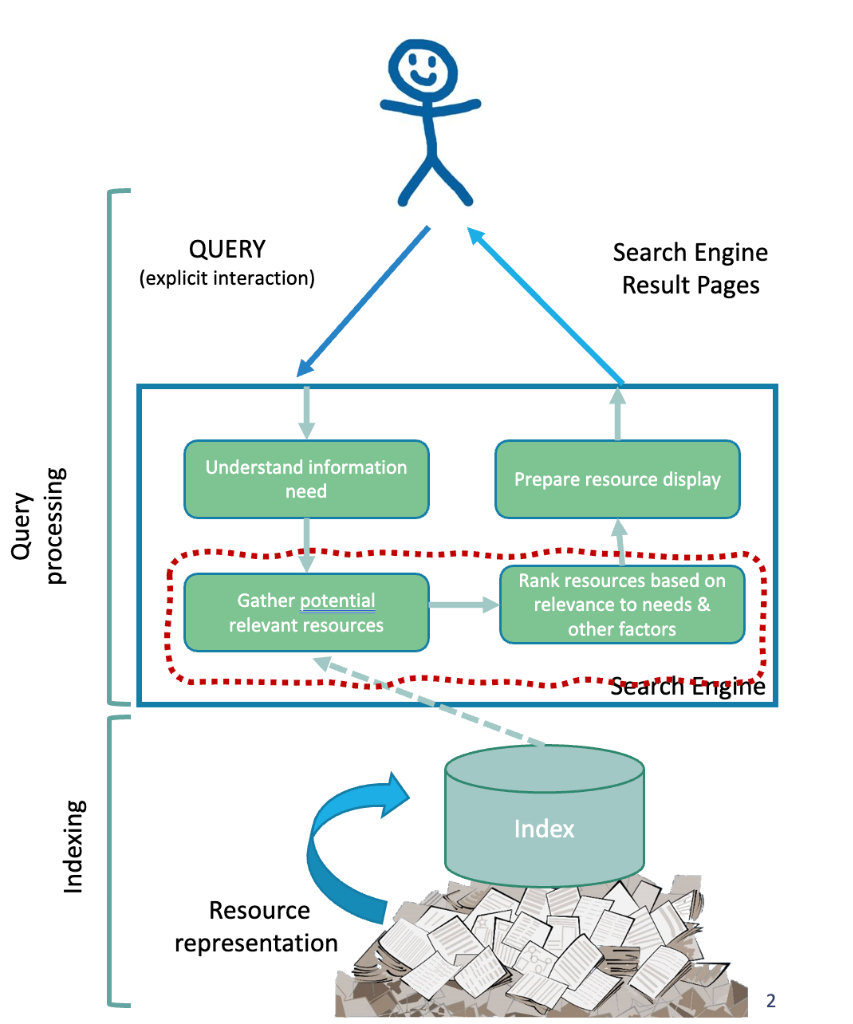
\includegraphics[width=0.7\textwidth]{figures/ir_pipeline.png}
\end{center}
\end{frame}

\begin{frame}[shrink=5]{Text Preprocessing \& Indexing}
\begin{block}{The Foundation of Search}
Building an IR system happens in three main stages:
\end{block}

\begin{itemize}
    \item \textbf{Stage 1: Offline Indexing}
    \begin{itemize}
        \item Documents are preprocessed (tokenized, stemmed, etc.)
        \item Inverted indexes are built and compressed
    \end{itemize}
    \item \textbf{Stage 2: Online Query Processing}
    \begin{itemize}
        \item Query is preprocessed \textbf{identically} to documents
        \item Match terms in the index
    \end{itemize}
    \item \textbf{Stage 3: Ranking}
    \begin{itemize}
        \item Scored according to a model (TF-IDF, BM25, etc.)
    \end{itemize}
\end{itemize}
\end{frame}

\begin{frame}[shrink=10]{Step-by-Step: Query Processing}
\textbf{Applying consistent preprocessing}

\vspace{1em}

\begin{exampleblock}{Example}
\textbf{User Query:} ``Running Dogs in the Park''

\vspace{0.5em}

\begin{enumerate}
    \item \textbf{Tokenization:} [Running, Dogs, in, the, Park]
    \item \textbf{Lowercasing:} [running, dogs, in, the, park]
    \item \textbf{Stop word removal:} [running, dogs, park]
    \item \textbf{Stemming:} [run, dog, park]
\end{enumerate}
\vspace{0.5em}

\textbf{Processed Query:} [run, dog, park]
\end{exampleblock}

\vspace{1em}

\begin{alertblock}{The Consistency Principle}
\textbf{Preprocessing must be identical for indexing and retrieval!}
\end{alertblock}
\end{frame}

\section{Inverted Index Posting Lists}

\begin{frame}{Inverted Index: Quick Recap}
\textbf{Core data structure for text search}

\vspace{1em}

\begin{center}
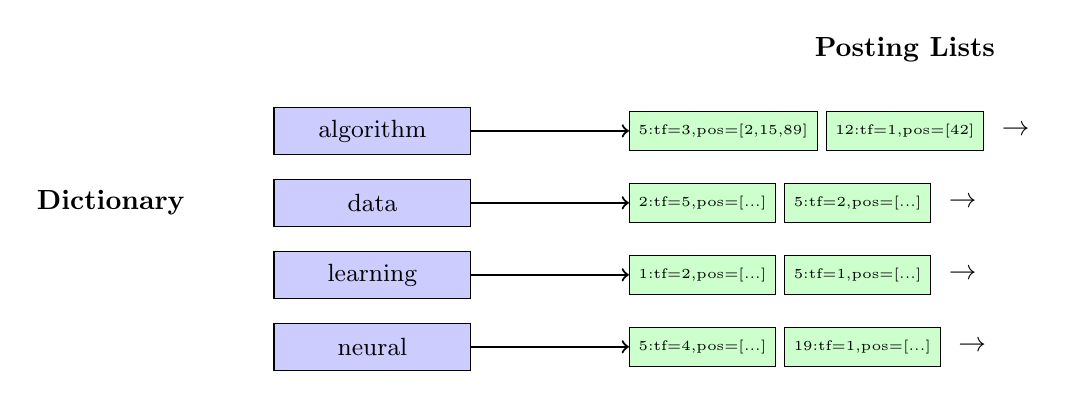
\begin{tikzpicture}[
    node distance=0.3cm,
    dict/.style={rectangle, draw, fill=blue!20, minimum width=2.5cm, minimum height=0.6cm, font=\small},
    post/.style={rectangle, draw, fill=green!20, minimum width=1.8cm, minimum height=0.5cm, font=\tiny}
]
    % Dictionary
    \node[dict] (term1) {algorithm};
    \node[dict, below=of term1] (term2) {data};
    \node[dict, below=of term2] (term3) {learning};
    \node[dict, below=of term3] (term4) {neural};
    
    \node[left=1cm of term2.west] {\textbf{Dictionary}};
    
    % Postings for "algorithm"
    \node[post, right=2cm of term1] (p11) {5:tf=3,pos=[2,15,89]};
    \node[post, right=0.1cm of p11] (p12) {12:tf=1,pos=[42]};
    \node[right=0.1cm of p12] {$\rightarrow$};
    
    % Postings for "data"
    \node[post, right=2cm of term2] (p21) {2:tf=5,pos=[...]};
    \node[post, right=0.1cm of p21] (p22) {5:tf=2,pos=[...]};
    \node[right=0.1cm of p22] {$\rightarrow$};
    
    % Postings for "learning"
    \node[post, right=2cm of term3] (p31) {1:tf=2,pos=[...]};
    \node[post, right=0.1cm of p31] (p32) {5:tf=1,pos=[...]};
    \node[right=0.1cm of p32] {$\rightarrow$};
    
    % Postings for "neural"
    \node[post, right=2cm of term4] (p41) {5:tf=4,pos=[...]};
    \node[post, right=0.1cm of p41] (p42) {19:tf=1,pos=[...]};
    \node[right=0.1cm of p42] {$\rightarrow$};
    
    \node[above=0.5cm of p12] {\textbf{Posting Lists}};
    
    % Arrows
    \draw[->, thick] (term1) -- (p11);
    \draw[->, thick] (term2) -- (p21);
    \draw[->, thick] (term3) -- (p31);
    \draw[->, thick] (term4) -- (p41);
\end{tikzpicture}
\end{center}

\vspace{1em}

\textbf{Each posting contains:}
\begin{itemize}
    \item Document ID \pause
    \item Term frequency (for ranking) \pause
    \item Positions (for phrase queries, proximity) \pause
    \item Potentially: field info, offsets, payload data
\end{itemize}
\end{frame}

\begin{frame}{Posting List Formats (1/2)}
\begin{block}{Basic Format: DocID Only}
$$\langle \text{docID}_1, \text{docID}_2, \text{docID}_3, \ldots \rangle$$
\begin{itemize}
    \item Minimal information
    \item Boolean queries only
    \item Example: [5, 12, 27, 89, 102]
\end{itemize}
\end{block}
\pause

\begin{block}{With Frequencies}
$$\langle (\text{docID}_1, \text{tf}_1), (\text{docID}_2, \text{tf}_2), \ldots \rangle$$
\begin{itemize}
    \item Enables TF-IDF, BM25 scoring
    \item Example: [(5, 3), (12, 1), (27, 2), (89, 1), (102, 5)]
\end{itemize}
\end{block}
\end{frame}

\begin{frame}{Posting List Formats (2/2)}
\begin{block}{With Positions (Full Inverted Index)}
$$\langle (\text{docID}_1, \text{tf}_1, [\text{pos}_{1,1}, \text{pos}_{1,2}, \ldots]), \ldots \rangle$$
\begin{itemize}
    \item Enables phrase queries, proximity scoring
    \item Example: [(5, 3, [2, 15, 89]), (12, 1, [42]), ...]
    \item Larger storage, but most flexible
\end{itemize}
\end{block}

\vspace{1em}

\textbf{Recommendation:} Use positions for production systems (enables phrase queries)
\end{frame}

\begin{frame}{Posting List Properties}
\begin{block}{Key Properties}
\begin{enumerate}
    \item \textbf{Sorted by DocID}
    \begin{itemize}
        \item Enables efficient merge operations
        \item Required for compression (gap encoding)
        \item Allows skip pointers
    \end{itemize}
    \pause
    
    \item \textbf{Variable Length}
    \begin{itemize}
        \item Rare terms: short lists (e.g., ``syzygy'': 10 docs)
        \item Common terms: long lists (e.g., ``the'': millions of docs)
        \item Power-law distribution (Zipf's law)
    \end{itemize}
    \pause
    
    \item \textbf{Stored Sequentially}
    \begin{itemize}
        \item Good cache locality
        \item Sequential disk reads (fast)
        \item Compressed for storage efficiency
    \end{itemize}
\end{enumerate}
\end{block}
\end{frame}

\begin{frame}{Skip Lists: Motivation}
\begin{alertblock}{Problem}
Merging long posting lists can be slow
\begin{itemize}
    \item Query: ``algorithm AND learning''
    \item ``algorithm'': 1M documents
    \item ``learning'': 500K documents
    \item Naive merge: scan both lists completely
\end{itemize}
\end{alertblock}

\vspace{1em}

\begin{exampleblock}{Example: Merging Without Skip Lists}
\textbf{List A:} [1, 5, 10, 15, 20, 25, 30, ...] (1M entries) \\
\textbf{List B:} [3, 6, 9, 12, 15, 18, 21, ...] (500K entries)

Finding intersection requires comparing \textbf{every} element: \\
Compare 1 vs 3, 5 vs 3, 5 vs 6, 10 vs 6, 10 vs 9, ...
\end{exampleblock}

\vspace{1em}

\begin{block}{Solution: Skip Pointers}
Add "shortcuts" to jump ahead in the list
\end{block}
\end{frame}

\begin{frame}{Skip Lists: Structure}
\begin{center}
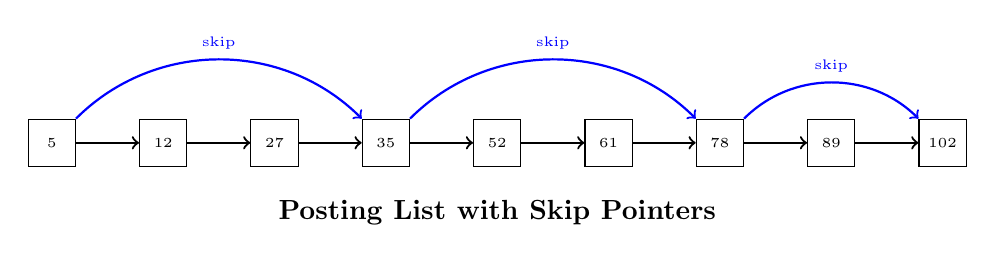
\begin{tikzpicture}[
    node distance=0.8cm,
    elem/.style={rectangle, draw, minimum width=0.6cm, minimum height=0.6cm, font=\tiny},
    skip/.style={->, thick, blue, bend left=45}
]
    % Bottom level (all elements)
    \node[elem] (e1) {5};
    \node[elem, right=of e1] (e2) {12};
    \node[elem, right=of e2] (e3) {27};
    \node[elem, right=of e3] (e4) {35};
    \node[elem, right=of e4] (e5) {52};
    \node[elem, right=of e5] (e6) {61};
    \node[elem, right=of e6] (e7) {78};
    \node[elem, right=of e7] (e8) {89};
    \node[elem, right=of e8] (e9) {102};
    
    % Regular pointers
    \draw[->, thick] (e1) -- (e2);
    \draw[->, thick] (e2) -- (e3);
    \draw[->, thick] (e3) -- (e4);
    \draw[->, thick] (e4) -- (e5);
    \draw[->, thick] (e5) -- (e6);
    \draw[->, thick] (e6) -- (e7);
    \draw[->, thick] (e7) -- (e8);
    \draw[->, thick] (e8) -- (e9);
    
    % Skip pointers (every 3 elements)
    \draw[skip] (e1) to node[above, font=\tiny] {skip} (e4);
    \draw[skip] (e4) to node[above, font=\tiny] {skip} (e7);
    \draw[skip] (e7) to node[above, font=\tiny] {skip} (e9);
    
    \node[below=0.3cm of e5] {\textbf{Posting List with Skip Pointers}};
\end{tikzpicture}
\end{center}

\vspace{1em}

\textbf{Skip pointers properties:}
\begin{itemize}
    \item Placed at regular intervals (e.g., every $\sqrt{n}$ elements)
    \item Point to future positions in the list
    \item Store the maximum docID they skip over
\end{itemize}

\vspace{0.5em}

\textbf{Trade-off:}
\begin{itemize}
    \item \textcolor{green}{\checkmark} Faster intersection (skip irrelevant parts)
    \item \textcolor{red}{\ding{55}} Extra storage for pointers
    \item \textcolor{red}{\ding{55}} Complexity in implementation
\end{itemize}
\end{frame}

\begin{frame}[shrink=5]{Skip Lists: Intersection Algorithm}
\begin{algorithmic}[1]
\STATE \textbf{Input:} Two posting lists $p_1, p_2$ with skip pointers
\STATE \textbf{Output:} Intersection of $p_1$ and $p_2$
\STATE
\STATE $i_1 \gets 0$, $i_2 \gets 0$ \COMMENT{Pointers to current positions}
\STATE $result \gets []$
\WHILE{$i_1 < |p_1|$ AND $i_2 < |p_2|$}
    \IF{$p_1[i_1].\text{docID} = p_2[i_2].\text{docID}$}
        \STATE Append $p_1[i_1].\text{docID}$ to $result$
        \STATE $i_1 \gets i_1 + 1$, $i_2 \gets i_2 + 1$
    \ELSIF{$p_1[i_1].\text{docID} < p_2[i_2].\text{docID}$}
        \IF{$p_1[i_1]$ has skip AND $p_1[i_1].\text{skip.maxDocID} \leq p_2[i_2].\text{docID}$}
            \STATE $i_1 \gets p_1[i_1].\text{skip}$ \COMMENT{Use skip pointer}
        \ELSE
            \STATE $i_1 \gets i_1 + 1$ \COMMENT{Advance normally}
        \ENDIF
    \ELSE
        \IF{$p_2[i_2]$ has skip AND $p_2[i_2].\text{skip.maxDocID} \leq p_1[i_1].\text{docID}$}
            \STATE $i_2 \gets p_2[i_2].\text{skip}$
        \ELSE
            \STATE $i_2 \gets i_2 + 1$
        \ENDIF
    \ENDIF
\ENDWHILE
\RETURN $result$
\end{algorithmic}
\end{frame}

\begin{frame}{Skip Lists: Example Intersection}
\textbf{Query:} Find intersection of two lists

\vspace{0.5em}

\textbf{List A:} [5, 12, 27, 35, 52, 61, 78, 89, 102] (skip every 3) \\
\textbf{List B:} [12, 35, 52, 89, 102, 150]

\vspace{1em}

\textbf{Trace:}
\begin{enumerate}
    \item Compare 5 vs 12 $\rightarrow$ 5 < 12, skip from 5 to 35
    \item Compare 35 vs 12 $\rightarrow$ 35 > 12, advance B to 35
    \item Compare 35 vs 35 $\rightarrow$ \textbf{Match!} $\rightarrow$ Output 35
    \item Compare 52 vs 52 $\rightarrow$ \textbf{Match!} $\rightarrow$ Output 52
    \item Compare 61 vs 89 $\rightarrow$ 61 < 89, skip from 61 to 89
    \item Compare 89 vs 89 $\rightarrow$ \textbf{Match!} $\rightarrow$ Output 89
    \item Compare 102 vs 102 $\rightarrow$ \textbf{Match!} $\rightarrow$ Output 102
    \item List A exhausted
\end{enumerate}

\vspace{1em}

\textbf{Result:} [35, 52, 89, 102]

\vspace{0.5em}

\textbf{Without skips:} 9 comparisons \\
\textbf{With skips:} 7 comparisons (used skip 2 times, saved 2 comparisons)
\end{frame}

\begin{frame}{Skip List Placement Strategy}
\begin{block}{How many skip pointers?}
Trade-off between space and speedup
\end{block}

\vspace{1em}

\textbf{Common strategies:}
\begin{enumerate}
    \item \textbf{$\sqrt{n}$ spacing} (optimal for random access)
    \begin{itemize}
        \item For list of length $n$, place $\sqrt{n}$ skip pointers
        \item Each skip jumps $\sqrt{n}$ positions
        \item Example: 10,000 elements $\rightarrow$ 100 skips, each spanning 100 elements
    \end{itemize}
    
    \item \textbf{Fixed interval} (simpler)
    \begin{itemize}
        \item Skip every $k$ elements (e.g., $k=10$)
        \item Easier to implement and maintain
    \end{itemize}
    
    \item \textbf{Multi-level skip lists}
    \begin{itemize}
        \item Skip pointers at multiple granularities
        \item Level 1: every 10, Level 2: every 100, etc.
        \item More complex but faster for very long lists
    \end{itemize}
\end{enumerate}

\vspace{1em}

\textbf{Typical choice:} Place skip every $\lfloor\sqrt{n}\rfloor$ elements
\end{frame}

% ====================================================================
% SECTION 2: QUERY PROCESSING ALGORITHMS
% ====================================================================
\section{Query Processing Algorithms}

\begin{frame}{Query Processing: The Task}
\begin{block}{Input}
\begin{itemize}
    \item Query: set of terms $q = \{t_1, t_2, \ldots, t_k\}$
    \item Inverted index with posting lists
    \item Scoring function (e.g., BM25, cosine similarity)
\end{itemize}
\end{block}

\begin{block}{Output}
\begin{itemize}
    \item Ranked list of top-$N$ documents by score
    \item Typically $N = 10$ or $N = 1000$
\end{itemize}
\end{block}

\vspace{1em}

\textbf{Key challenge:} Efficiency
\begin{itemize}
    \item Can't score all documents (millions/billions) \pause
    \item Must process posting lists cleverly \pause
    \item Different algorithms for different scenarios
\end{itemize}
\end{frame}

\begin{frame}{Two Main Paradigms}
\begin{columns}
\begin{column}{0.48\textwidth}
\begin{block}{Document-at-a-Time (DAAT)}
\begin{itemize}
    \item Process one document completely
    \item Compute full score for that doc
    \item Move to next document
    \item Keep top-$k$ heap
\end{itemize}

\vspace{0.5em}

\textbf{Analogy:} Grading exams
\begin{itemize}
    \item Grade all questions for student 1
    \item Then all questions for student 2
    \item Etc.
\end{itemize}
\end{block}
\end{column}

\begin{column}{0.48\textwidth}
\begin{block}{Term-at-a-Time (TAAT)}
\begin{itemize}
    \item Process one query term completely
    \item Update partial scores for all docs
    \item Move to next query term
    \item Accumulate scores
\end{itemize}

\vspace{0.5em}

\textbf{Analogy:} Grading exams
\begin{itemize}
    \item Grade question 1 for all students
    \item Then question 2 for all students
    \item Etc.
\end{itemize}
\end{block}
\end{column}
\end{columns}

\vspace{1em}

\begin{alertblock}{Which is better?}
Depends on: query length, list lengths, scoring function, hardware
\end{alertblock}
\end{frame}

\begin{frame}{Document-at-a-Time (DAAT)}
\begin{algorithmic}[1]
\STATE \textbf{Input:} Query terms $\{t_1, t_2, \ldots, t_k\}$, posting lists
\STATE \textbf{Output:} Top-$N$ documents
\STATE
\STATE Fetch posting lists for all query terms
\STATE $\text{heap} \gets$ empty min-heap of size $N$ \COMMENT{Store top-N docs}
\STATE $\text{nextDocID} \gets$ minimum docID across all posting lists
\WHILE{posting lists not exhausted}
    \STATE $d \gets \text{nextDocID}$
    \STATE $\text{score} \gets 0$
    \FOR{each term $t_i$ in query}
        \IF{$t_i$'s posting list contains $d$}
            \STATE $\text{score} \gets \text{score} + \text{termScore}(t_i, d)$ \COMMENT{BM25, TF-IDF, etc.}
            \STATE Advance $t_i$'s pointer
        \ENDIF
    \ENDFOR
    \STATE Add $(d, \text{score})$ to heap (evict min if heap full)
    \STATE $\text{nextDocID} \gets$ next minimum docID across all lists
\ENDWHILE
\RETURN top-$N$ from heap
\end{algorithmic}
\end{frame}

\begin{frame}{DAAT Example}
\textbf{Query:} ``neural learning'' \\
\textbf{Posting lists:}
\begin{itemize}
    \item neural: [5, 12, 27, 89]
    \item learning: [5, 27, 35, 89]
\end{itemize}

\vspace{1em}

\textbf{Processing (top-2):}
\begin{enumerate}
    \item \textbf{Doc 5:} Both terms present $\rightarrow$ score = $\text{BM25}(\text{neural}, 5) + \text{BM25}(\text{learning}, 5) = 2.3$
    \begin{itemize}
        \item Heap: [(5, 2.3)]
    \end{itemize}
    
    \item \textbf{Doc 12:} Only ``neural'' $\rightarrow$ score = $\text{BM25}(\text{neural}, 12) = 1.1$
    \begin{itemize}
        \item Heap: [(5, 2.3), (12, 1.1)]
    \end{itemize}
    
    \item \textbf{Doc 27:} Both terms $\rightarrow$ score = $3.1$
    \begin{itemize}
        \item Heap: [(5, 2.3), (27, 3.1)] (evict doc 12)
    \end{itemize}
    
    \item \textbf{Doc 35:} Only ``learning'' $\rightarrow$ score = $0.9$
    \begin{itemize}
        \item Heap unchanged (score too low)
    \end{itemize}
    
    \item \textbf{Doc 89:} Both terms $\rightarrow$ score = $2.5$
    \begin{itemize}
        \item Heap: [(27, 3.1), (89, 2.5)] (evict doc 5)
    \end{itemize}
\end{enumerate}

\textbf{Final result:} [27, 89]
\end{frame}

\begin{frame}{DAAT with Skip Pointers}
\textbf{Optimization:} Use skip pointers to jump to next candidate document

\vspace{1em}

\begin{algorithmic}[1]
\STATE Find document $d$ that appears in \textit{at least one} posting list
\IF{$d$ appears in all posting lists}
    \STATE Compute full score for $d$
\ELSIF{$d$ appears in some but not all lists}
    \STATE Compute partial score for $d$ (only from matching terms)
\ENDIF
\STATE Use skip pointers to advance to next candidate efficiently
\end{algorithmic}

\vspace{1em}

\textbf{Key insight:}
\begin{itemize}
    \item Shortest posting list determines candidates
    \item Use skips to align longer lists to candidates
    \item Much faster when lists have very different lengths
\end{itemize}

\vspace{1em}

\textbf{Example:}
\begin{itemize}
    \item Query: ``rare common''
    \item ``rare'': [5, 89] (2 docs)
    \item ``common'': [1, 2, 3, ..., 1000000] (1M docs)
    \item Only score docs 5 and 89 (use skips to find them in ``common'')
\end{itemize}
\end{frame}

\begin{frame}{Term-at-a-Time (TAAT)}
\begin{algorithmic}[1]
\STATE \textbf{Input:} Query terms $\{t_1, t_2, \ldots, t_k\}$, posting lists
\STATE \textbf{Output:} Top-$N$ documents
\STATE
\STATE $\text{scores} \gets$ empty hash table (docID $\rightarrow$ score)
\FOR{each query term $t_i$}
    \STATE Fetch posting list for $t_i$
    \FOR{each document $d$ in posting list}
        \IF{$d$ not in scores}
            \STATE $\text{scores}[d] \gets 0$
        \ENDIF
        \STATE $\text{scores}[d] \gets \text{scores}[d] + \text{termScore}(t_i, d)$
    \ENDFOR
\ENDFOR
\STATE Sort documents by score (descending)
\RETURN top-$N$ documents
\end{algorithmic}

\vspace{1em}

\textbf{Note:} All documents get partial scores as we go; final scores computed after processing all terms
\end{frame}

\begin{frame}{TAAT Example}
\textbf{Query:} ``neural learning'' \\
\textbf{Posting lists:}
\begin{itemize}
    \item neural: [5, 12, 27, 89]
    \item learning: [5, 27, 35, 89]
\end{itemize}

\vspace{1em}

\textbf{Processing:}

\textbf{Step 1: Process ``neural''}
\begin{itemize}
    \item Doc 5: scores[5] = 1.5
    \item Doc 12: scores[12] = 1.1
    \item Doc 27: scores[27] = 1.6
    \item Doc 89: scores[89] = 1.3
\end{itemize}

\textbf{Step 2: Process ``learning''}
\begin{itemize}
    \item Doc 5: scores[5] = 1.5 + 0.8 = 2.3
    \item Doc 27: scores[27] = 1.6 + 1.5 = 3.1
    \item Doc 35: scores[35] = 0.9
    \item Doc 89: scores[89] = 1.3 + 1.2 = 2.5
\end{itemize}

\vspace{1em}

\textbf{Final scores:} \{5: 2.3, 12: 1.1, 27: 3.1, 35: 0.9, 89: 2.5\} \\
\textbf{Sorted:} [27, 89, 5, 12, 35] \\
\textbf{Top-2:} [27, 89]
\end{frame}

\begin{frame}{DAAT vs. TAAT Comparison}
\begin{table}
\centering
\small
\begin{tabular}{lll}
\toprule
\textbf{Aspect} & \textbf{DAAT} & \textbf{TAAT} \\
\midrule
Memory & Low (only top-$k$ heap) & High (all candidate scores) \\
Cache locality & Good (sequential per doc) & Poor (random access) \\
Early termination & Easy (threshold pruning) & Hard (need all terms) \\
Parallelization & Harder & Easier (independent terms) \\
Skip pointers & Very effective & Less effective \\
Long queries & Better & Worse (more memory) \\
Conjunctive queries & Natural & Must filter at end \\
\midrule
\textbf{Modern systems} & \textbf{Preferred} & Used in batch scoring \\
\bottomrule
\end{tabular}
\end{table}

\vspace{1em}

\begin{block}{Practical Choice}
\begin{itemize}
    \item \textbf{DAAT:} Most production systems (Lucene, Elasticsearch, Solr)
    \item \textbf{TAAT:} Batch re-ranking, research systems
    \item \textbf{Hybrid:} Process short lists DAAT, long lists TAAT
\end{itemize}
\end{block}
\end{frame}

\begin{frame}{Query Optimization: MaxScore}
\begin{block}{Observation}
Not all query terms contribute equally to final scores
\end{block}

\vspace{1em}

\textbf{MaxScore Algorithm:}
\begin{enumerate}
    \item Compute maximum possible contribution for each term
    $$\text{maxScore}(t) = \max_{d} \text{score}(t, d)$$
    
    \item Sort query terms by maxScore (descending)
    
    \item Maintain threshold $\theta$ = score of $k$-th best document so far
    
    \item Skip processing term $t$ for document $d$ if:
    $$\text{score}(d) + \text{maxScore}(t) < \theta$$
    (Can't possibly make top-$k$)
\end{enumerate}

\vspace{1em}

\textbf{Result:} Avoid scoring low-impact terms for documents that won't reach top-$k$
\end{frame}

\begin{frame}{MaxScore Example}
\textbf{Query:} ``neural network learning''

\vspace{0.5em}

\textbf{Max scores:}
\begin{itemize}
    \item neural: maxScore = 2.5
    \item network: maxScore = 2.0
    \item learning: maxScore = 1.5
\end{itemize}

\textbf{Sorted by maxScore:} [neural, network, learning]

\vspace{1em}

\textbf{Processing doc 42 (top-10 query):}
\begin{enumerate}
    \item Current 10th-best score: $\theta = 5.0$
    \item Score so far for doc 42: $3.0$ (from ``neural'' and ``network'')
    \item Max additional score: $1.5$ (from ``learning'')
    \item Total possible: $3.0 + 1.5 = 4.5 < 5.0$
    \item \textbf{Skip} scoring ``learning'' for doc 42 (can't reach top-10)
\end{enumerate}

\vspace{1em}

\begin{block}{Benefit}
Saves scoring effort for documents that won't make top-$k$ \\
Especially effective for long queries
\end{block}
\end{frame}

\begin{frame}{Query Optimization: WAND}
\begin{block}{Weak AND (WAND)}
Advanced optimization combining DAAT with dynamic pruning
\end{block}

\vspace{1em}

\textbf{Key ideas:}
\begin{enumerate}
    \item Maintain upper bounds on term contributions
    \item Process posting lists in parallel (like DAAT)
    \item Skip entire documents if upper bound < threshold
    \item Dynamically update threshold as better docs found
\end{enumerate}

\vspace{1em}

\textbf{WAND pivot algorithm:}
\begin{itemize}
    \item Find "pivot" document where sum of upper bounds $\geq \theta$
    \item All documents before pivot can be safely skipped
    \item Use skip pointers to jump to pivot
\end{itemize}

\vspace{1em}

\begin{exampleblock}{Performance}
\begin{itemize}
    \item Can skip 90-99\% of postings for top-10 queries
    \item 10-100$\times$ speedup vs. naive DAAT
    \item Used in production systems (e.g., Lucene 8+)
\end{itemize}
\end{exampleblock}
\end{frame}

\begin{frame}{Impact-Ordered Indexes}
\begin{block}{Alternative Index Organization}
Instead of sorting postings by docID, sort by impact (score)
\end{block}

\vspace{1em}

\textbf{Traditional (docID-ordered):}
\begin{itemize}
    \item neural: [(5, tf=1), (12, tf=3), (27, tf=1), (89, tf=5)]
    \item Sorted by docID
\end{itemize}

\vspace{0.5em}

\textbf{Impact-ordered:}
\begin{itemize}
    \item neural: [(89, tf=5), (12, tf=3), (5, tf=1), (27, tf=1)]
    \item Sorted by term frequency (or TF-IDF score)
\end{itemize}

\vspace{1em}

\textbf{Benefits:}
\begin{itemize}
    \item \textbf{Early termination:} Stop after processing top-$k$ high-impact postings \pause
    \item \textbf{Safe to skip:} Low-impact docs unlikely to reach top-$k$ \pause
    \item \textbf{Query-independent:} Pre-computed at index time
\end{itemize}
\pause

\vspace{0.5em}

\textbf{Drawback:}
\begin{itemize}
    \item Can't use skip pointers (not sorted by docID) \pause
    \item Boolean queries harder (need docID order for AND)
\end{itemize}
\end{frame}

% ====================================================================
% SECTION 3: INDEX COMPRESSION
% ====================================================================
\section{Index Compression}

\begin{frame}{Why Compress Indexes?}
\begin{block}{Motivation}
\begin{enumerate}
    \item \textbf{Storage costs}
    \begin{itemize}
        \item Uncompressed index: 10-20\% of raw collection size
        \item For 100TB collection: 10-20TB index
        \item Compression: 5-10$\times$ reduction $\rightarrow$ 1-4TB
    \end{itemize}
    
    \item \textbf{I/O efficiency}
    \begin{itemize}
        \item Disk/SSD bandwidth: 500 MB/s
        \item Decompression: 2-5 GB/s
        \item Reading compressed data is \textbf{faster}!
    \end{itemize}
    
    \item \textbf{Cache efficiency}
    \begin{itemize}
        \item More index fits in RAM
        \item Better cache hit rates
        \item Faster query processing
    \end{itemize}
\end{enumerate}
\end{block}

\vspace{1em}

\begin{alertblock}{Key Principle}
Disk is slow, CPU is fast $\rightarrow$ compression almost always wins
\end{alertblock}
\end{frame}

\begin{frame}{What to Compress?}
\begin{columns}
\begin{column}{0.48\textwidth}
\begin{block}{Dictionary}
\textbf{Size:} 100-500 MB (small) \\
\textbf{Techniques:}
\begin{itemize}
    \item Front coding
    \item Suffix arrays
    \item Finite-state automata
\end{itemize}
\textbf{Impact:} Minor (already small)
\end{block}
\end{column}

\begin{column}{0.48\textwidth}
\begin{block}{Postings Lists}
\textbf{Size:} Gigabytes to terabytes \\
\textbf{Techniques:}
\begin{itemize}
    \item Gap encoding
    \item Variable-byte
    \item Gamma/Delta codes
    \item PForDelta
\end{itemize}
\textbf{Impact:} \textbf{Major} (most of index)
\end{block}
\end{column}
\end{columns}

\vspace{1em}

\begin{exampleblock}{Typical Index Breakdown}
\begin{itemize}
    \item Dictionary: 2\%
    \item Postings (docIDs): 70\%
    \item Postings (frequencies): 10\%
    \item Postings (positions): 18\%
\end{itemize}
$\rightarrow$ Focus compression on docIDs and positions!
\end{exampleblock}
\end{frame}

\begin{frame}{Dictionary Compression: Front Coding}
\begin{block}{Observation}
Sorted dictionary has many shared prefixes
\end{block}

\vspace{1em}

\begin{columns}
\begin{column}{0.48\textwidth}
\textbf{Uncompressed:}
\begin{itemize}
    \item[] \texttt{algorithm}
    \item[] \texttt{algorithmic}
    \item[] \texttt{algorithmically}
    \item[] \texttt{algorithms}
    \item[] \texttt{alien}
    \item[] \texttt{align}
    \item[] \texttt{alignment}
\end{itemize}

\textbf{Storage:} 64 bytes
\end{column}

\begin{column}{0.48\textwidth}
\textbf{Front coded:}
\begin{itemize}
    \item[] \texttt{9 algorithm}
    \item[] \texttt{~~2 ic}
    \item[] \texttt{~~5 ally}
    \item[] \texttt{~~1 s}
    \item[] \texttt{5 ali}
    \item[] \texttt{~~2 en}
    \item[] \texttt{~~2 gn}
    \item[] \texttt{~~5 ment}
\end{itemize}

\textbf{Storage:} $\approx$ 38 bytes \\
\textbf{Savings:} 40\%
\end{column}
\end{columns}

\vspace{1em}

\textbf{Format:} (prefix\_length, suffix) \\
\textbf{Block size:} Typically reset every 8-16 terms for random access
\end{frame}

\begin{frame}{Postings Compression: Gap Encoding}
\begin{block}{Key Insight}
DocIDs in postings are sorted $\rightarrow$ store gaps instead of absolute values
\end{block}

\vspace{1em}

\textbf{Original postings (docIDs):}
$$[5, 127, 214, 215, 512, 1024, 2048, 10239]$$

\vspace{0.5em}

\textbf{Gaps (d-gaps):}
$$[5, 122, 87, 1, 297, 512, 1024, 8191]$$

\vspace{1em}

\begin{exampleblock}{Why This Helps}
\begin{itemize}
    \item \textbf{Original:} Numbers range from 5 to 10,239 (need 14 bits each)
    \item \textbf{Gaps:} Most numbers small (need fewer bits)
    \item Small numbers compress much better!
\end{itemize}
\end{exampleblock}

\vspace{1em}

\begin{alertblock}{Critical Property}
Can decode sequentially: \\
$\text{docID}_i = \text{docID}_{i-1} + \text{gap}_i$ (starting from 0)
\end{alertblock}
\end{frame}

\begin{frame}{Gap Distribution}
\begin{block}{Zipf's Law}
Term frequencies follow power-law distribution
\end{block}

\vspace{1em}

\textbf{Implications for gaps:}
\begin{itemize}
    \item \textbf{Rare terms:} Large gaps (appear infrequently)
    \item \textbf{Common terms:} Small gaps (appear often)
    \item \textbf{Overall:} Most gaps are small!
\end{itemize}

\vspace{1em}

\begin{exampleblock}{Example}
\textbf{Rare term ``syzygy'':} [15, 5023, 89234] \\
Gaps: [15, 5008, 84211] (large gaps)

\vspace{0.5em}

\textbf{Common term ``the'':} [1, 2, 5, 7, 8, 10, 12, ...] \\
Gaps: [1, 1, 3, 2, 1, 2, 2, ...] (small gaps)
\end{exampleblock}

\vspace{1em}

\textbf{Goal:} Use fewer bits for small numbers, more bits for large numbers
\end{frame}

\begin{frame}{Variable Byte (VB) Encoding}
\begin{block}{Core Idea}
Use variable number of bytes to encode integers
\begin{itemize}
    \item Small numbers: 1 byte
    \item Larger numbers: 2+ bytes
    \item Self-delimiting: continuation bit indicates if more bytes follow
\end{itemize}
\end{block}

\vspace{1em}

\textbf{Encoding scheme:}
\begin{itemize}
    \item Use 7 bits per byte for data
    \item Use 1 bit (MSB) as continuation flag
    \item 1 = last byte, 0 = more bytes follow
\end{itemize}

\vspace{1em}

\begin{table}
\centering
\small
\begin{tabular}{lll}
\toprule
\textbf{Number} & \textbf{Binary} & \textbf{VB Encoding} \\
\midrule
5 & 101 & \texttt{1\_0000101} (1 byte) \\
130 & 10000010 & \texttt{0\_0000001 1\_0000010} (2 bytes) \\
16383 & 11111111111111 & \texttt{0\_1111111 1\_1111111} (2 bytes) \\
\bottomrule
\end{tabular}
\end{table}

\textbf{Note:} Underscore separates continuation bit from data bits
\end{frame}

\begin{frame}{VB Encoding: Detailed Examples}
\textbf{Example 1: Encode 5}
\begin{enumerate}
    \item Binary: 101 (3 bits)
    \item Fits in 7 bits $\rightarrow$ use 1 byte
    \item Data: 0000101, continuation: 1 (last byte)
    \item Result: \texttt{10000101}
\end{enumerate}

\vspace{1em}

\textbf{Example 2: Encode 824}
\begin{enumerate}
    \item Binary: 1100111000 (10 bits)
    \item Needs 2 bytes (10 > 7)
    \item Split into 7-bit chunks (from right): 0111000, 0000110
    \item First byte (higher bits): 0\_0000110 (more bytes follow)
    \item Second byte (lower bits): 1\_0111000 (last byte)
    \item Result: \texttt{00000110 10111000}
\end{enumerate}

\vspace{1em}

\textbf{Decoding:}
\begin{enumerate}
    \item Read bytes until continuation bit = 1
    \item Strip continuation bits
    \item Concatenate data bits
    \item Convert to integer
\end{enumerate}
\end{frame}

\begin{frame}{VB: Compressing a Posting List}
\textbf{Original docIDs:} [5, 127, 214, 215]

\vspace{0.5em}

\textbf{Step 1: Compute gaps}
\begin{itemize}
    \item Gap 1: 5 - 0 = 5
    \item Gap 2: 127 - 5 = 122
    \item Gap 3: 214 - 127 = 87
    \item Gap 4: 215 - 214 = 1
\end{itemize}
Gaps: [5, 122, 87, 1]

\vspace{1em}

\textbf{Step 2: VB encode each gap}
\begin{itemize}
    \item 5 $\rightarrow$ \texttt{10000101} (1 byte)
    \item 122 $\rightarrow$ \texttt{11111010} (1 byte)
    \item 87 $\rightarrow$ \texttt{11010111} (1 byte)
    \item 1 $\rightarrow$ \texttt{10000001} (1 byte)
\end{itemize}

\vspace{1em}

\textbf{Result:} 4 bytes compressed vs. 16 bytes uncompressed (32-bit ints)

\textbf{Compression ratio:} 4$\times$ \\
\textbf{Decompression:} Very fast (byte-aligned, simple bit ops)
\end{frame}

\begin{frame}{Gamma Encoding}
\begin{block}{Motivation}
VB uses 8 bits to encode 7 bits (12.5\% overhead) \\
Can we do better for very small numbers?
\end{block}

\vspace{1em}

\textbf{Gamma encoding:}
\begin{enumerate}
    \item Let $N = \lfloor \log_2 x \rfloor$ (position of highest bit)
    \item Encode $N$ in unary: $N$ zeros + one 1
    \item Encode offset $x - 2^N$ in $N$ bits
\end{enumerate}

\vspace{1em}

\begin{exampleblock}{Examples}
\textbf{Encode 5:}
\begin{itemize}
    \item Binary: 101, $N = 2$ (highest bit at position 2)
    \item Unary for $N=2$: 001 (two zeros + 1)
    \item Offset: $5 - 2^2 = 1$ $\rightarrow$ 01 (in 2 bits)
    \item Result: \texttt{00101} (5 bits total)
\end{itemize}

\textbf{Encode 13:}
\begin{itemize}
    \item Binary: 1101, $N = 3$
    \item Unary for $N=3$: 0001
    \item Offset: $13 - 2^3 = 5$ $\rightarrow$ 101 (in 3 bits)
    \item Result: \texttt{0001101} (7 bits total)
\end{itemize}
\end{exampleblock}
\end{frame}

\begin{frame}{Gamma Encoding: More Examples}
\begin{table}
\centering
\small
\begin{tabular}{lcccl}
\toprule
\textbf{$x$} & \textbf{Binary} & \textbf{$N$} & \textbf{Offset} & \textbf{Gamma Code} \\
\midrule
1 & 1 & 0 & 0 & \texttt{1} (1 bit) \\
2 & 10 & 1 & 0 & \texttt{010} (3 bits) \\
3 & 11 & 1 & 1 & \texttt{011} (3 bits) \\
4 & 100 & 2 & 0 & \texttt{00100} (5 bits) \\
5 & 101 & 2 & 1 & \texttt{00101} (5 bits) \\
9 & 1001 & 3 & 1 & \texttt{0001001} (7 bits) \\
100 & 1100100 & 6 & 36 & \texttt{000000\_1100100} (13 bits) \\
\bottomrule
\end{tabular}
\end{table}

\vspace{1em}

\textbf{Observations:}
\begin{itemize}
    \item Very efficient for small numbers (1-15)
    \item Encoding length: $2\lfloor \log_2 x \rfloor + 1$ bits
    \item Self-delimiting (no need for length prefix)
    \item Optimal for geometric distributions
\end{itemize}
\end{frame}

\begin{frame}{VB vs. Gamma Comparison}
\begin{table}
\centering
\small
\begin{tabular}{lccc}
\toprule
\textbf{Number} & \textbf{VB (bits)} & \textbf{Gamma (bits)} & \textbf{Better} \\
\midrule
1 & 8 & 1 & Gamma \\
5 & 8 & 5 & Gamma \\
10 & 8 & 7 & Gamma \\
100 & 8 & 13 & VB \\
127 & 8 & 13 & VB \\
128 & 16 & 15 & Gamma \\
1000 & 16 & 19 & VB \\
10000 & 16 & 27 & VB \\
\bottomrule
\end{tabular}
\end{table}

\vspace{1em}

\begin{block}{Trade-offs}
\begin{itemize}
    \item \textbf{Gamma:} Better compression for numbers < 128
    \item \textbf{VB:} Simpler, faster, better for larger numbers
    \item \textbf{Gamma:} Requires bit-level operations (slower)
    \item \textbf{VB:} Byte-aligned (faster on modern hardware)
\end{itemize}
\end{block}

\textbf{Practical choice:} VB dominates in production systems (speed wins)
\end{frame}

\begin{frame}{PForDelta: Patched Frame of Reference}
\begin{block}{Key Observation}
In most posting lists, the vast majority of gaps fit in a small number of bits, but a few outliers are much larger
\end{block}

\vspace{1em}

\textbf{PForDelta idea:}
\begin{enumerate}
    \item Divide postings into blocks (e.g., 128 values)
    \item Choose bit width $b$ that fits 90\% of values in block
    \item Store majority in $b$ bits each (packed tightly)
    \item Store exceptions separately with positions
\end{enumerate}

\vspace{1em}

\begin{exampleblock}{Example}
\textbf{Gaps:} [5, 3, 7, 512, 2, 4, 1, 6, 9, 3]

\begin{itemize}
    \item Choose $b=3$ bits (fits all except 512)
    \item Main array: [5, 3, 7, \textcolor{red}{0}, 2, 4, 1, 6, 9, 3] (3 bits each = 30 bits)
    \item Exceptions: Position 3 $\rightarrow$ value 512
    \item Total: 30 bits + exception overhead vs. 10$\times$ log-encoding
\end{itemize}
\end{exampleblock}
\end{frame}

\begin{frame}{PForDelta: Detailed Algorithm}
\textbf{Encoding:}
\begin{algorithmic}[1]
\STATE Divide gaps into blocks of size $B$ (e.g., 128)
\FOR{each block}
    \STATE Compute histogram of gap values
    \STATE Choose $b$ such that $\geq 90\%$ of values fit in $b$ bits
    \STATE Pack values that fit into $b$-bit array
    \STATE For exceptions (values $\geq 2^b$):
        \STATE \quad Store position in block
        \STATE \quad Store actual value separately
        \STATE \quad Put special marker in main array
    \STATE Store: $b$, packed array, exception list
\ENDFOR
\end{algorithmic}

\vspace{1em}

\textbf{Decoding:}
\begin{enumerate}
    \item Read $b$ (bit width)
    \item Unpack $b$-bit values from packed array
    \item Patch in exceptions at their positions
    \item Reconstruct docIDs from gaps
\end{enumerate}
\end{frame}

\begin{frame}{PForDelta: Performance}
\begin{block}{Advantages}
\begin{itemize}
    \item \textbf{Excellent compression:} 5-10$\times$ typical
    \item \textbf{Very fast decompression:} SIMD-friendly (process 128 bits at once)
    \item \textbf{Random access:} Can decode individual blocks
    \item \textbf{Adaptive:} Bit width chosen per block
\end{itemize}
\end{block}

\begin{alertblock}{Disadvantages}
\begin{itemize}
    \item \textbf{Complex implementation:} Bit packing, exception handling
    \item \textbf{Block-based:} Small overhead for block headers
    \item \textbf{Not universal:} Requires careful tuning
\end{itemize}
\end{alertblock}

\vspace{1em}

\begin{exampleblock}{Typical Performance}
\begin{itemize}
    \item Compression: 6-8$\times$ for typical web collections
    \item Decompression: 3-5 GB/s on modern CPU
    \item Used in: Lucene, Elasticsearch (via FOR variants)
\\end{itemize}
\end{exampleblock}
\end{frame}

\begin{frame}{Compression Method Summary}
\begin{table}
\centering
\footnotesize
\begin{tabular}{lcccc}
\toprule
\textbf{Method} & \textbf{Compression} & \textbf{Dec. Speed} & \textbf{Complexity} & \textbf{Use Case} \\
\midrule
None & 1$\times$ & Fastest & Trivial & Small indexes \\
VB & 3-4$\times$ & Fast & Simple & General purpose \\
Gamma & 4-5$\times$ & Medium & Moderate & Small gaps \\
PForDelta & 6-10$\times$ & Very Fast & Complex & Production \\
Simple-9/16 & 4-6$\times$ & Very Fast & Moderate & Production \\
\bottomrule
\end{tabular}
\end{table}

\vspace{1em}

\begin{block}{Recommendations}
\begin{itemize}
    \item \textbf{Learning/prototyping:} Start with VB (easy to implement)
    \item \textbf{Production (small/medium):} VB (good enough, simple)
    \item \textbf{Production (large scale):} PForDelta or Simple-16 (best performance)
    \item \textbf{Research:} Experiment with adaptive schemes
\end{itemize}
\end{block}

\vspace{1em}

\begin{alertblock}{Modern Trend}
Increasingly sophisticated compression + SIMD decompression \\
Example: Lucene uses FOR (Frame of Reference) with SIMD
\end{alertblock}
\end{frame}

% ====================================================================
% SECTION 4: APPROXIMATE K-NN INDEXING
% ====================================================================
\section{Approximate k-NN Indexing for Dense Retrieval}

\begin{frame}{From Sparse to Dense Retrieval}
\begin{columns}
\begin{column}{0.48\textwidth}
\begin{block}{Sparse (Traditional)}
\textbf{Representation:}
\begin{itemize}
    \item Bag of words
    \item High-dimensional (vocab size)
    \item Mostly zeros (99\%+ sparse)
\end{itemize}

\textbf{Index:} Inverted index

\textbf{Search:} AND/OR logic, BM25

\textbf{Limitation:} Vocabulary mismatch
\end{block}
\end{column}

\begin{column}{0.48\textwidth}
\begin{block}{Dense (Neural)}
\textbf{Representation:}
\begin{itemize}
    \item Learned embeddings
    \item Low-dimensional (100-1000d)
    \item All non-zero (dense)
\end{itemize}

\textbf{Index:} Vector database

\textbf{Search:} Nearest neighbors

\textbf{Advantage:} Semantic matching
\end{block}
\end{column}
\end{columns}

\vspace{1em}

\begin{exampleblock}{Example}
\textbf{Query:} ``car problems'' \\
\textbf{Sparse:} Misses document with ``automobile issues'' \\
\textbf{Dense:} Finds it! (similar embeddings)
\end{exampleblock}
\end{frame}

\begin{frame}{Dense Retrieval: The Pipeline}
\begin{center}
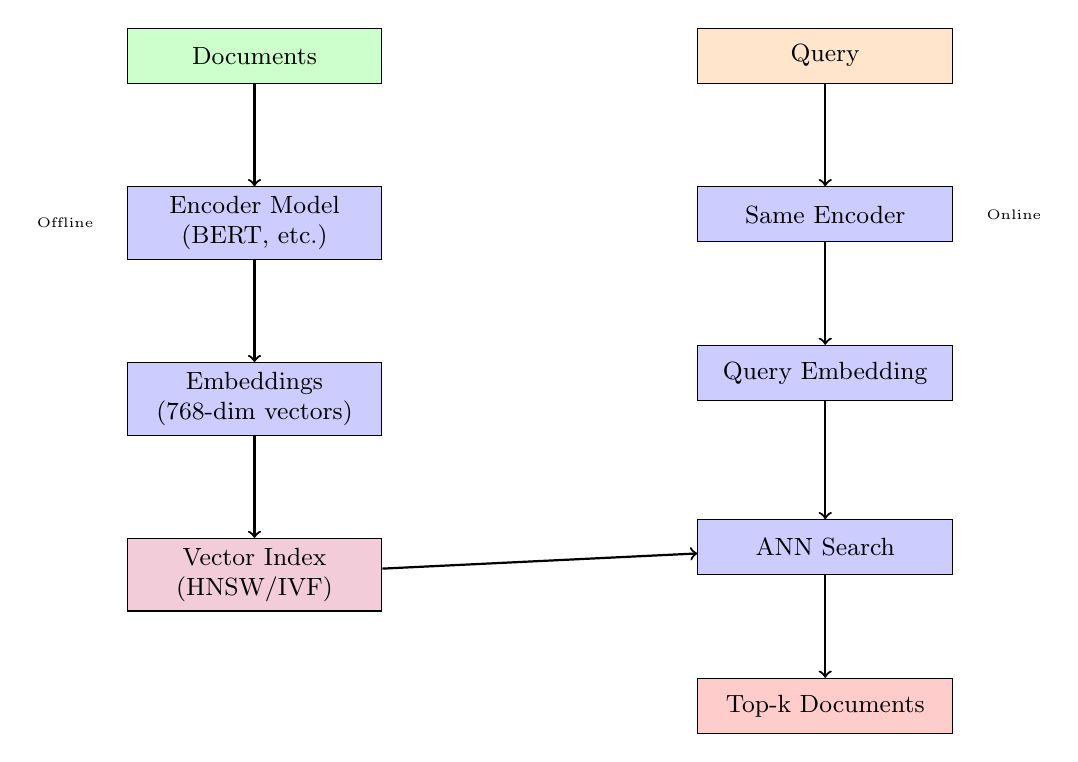
\begin{tikzpicture}[
    node distance=1.3cm,
    box/.style={rectangle, draw, fill=blue!20, text width=3cm, align=center, minimum height=0.7cm, font=\small},
    arrow/.style={->, thick}
]
    % Offline indexing
    \node[box, fill=green!20] (docs) {Documents};
    \node[box, below=of docs] (encoder) {Encoder Model \\ (BERT, etc.)};
    \node[box, below=of encoder] (embed) {Embeddings \\ (768-dim vectors)};
    \node[box, below=of embed, fill=purple!20] (index) {Vector Index \\ (HNSW/IVF)};
    
    % Online query
    \node[box, right=4cm of docs, fill=orange!20] (query) {Query};
    \node[box, below=of query] (qencoder) {Same Encoder};
    \node[box, below=of qencoder] (qembed) {Query Embedding};
    
    % Search
    \node[box, below=1.5cm of qembed] (search) {ANN Search};
    \node[box, below=of search, fill=red!20] (results) {Top-k Documents};
    
    % Arrows
    \draw[arrow] (docs) -- (encoder);
    \draw[arrow] (encoder) -- (embed);
    \draw[arrow] (embed) -- (index);
    
    \draw[arrow] (query) -- (qencoder);
    \draw[arrow] (qencoder) -- (qembed);
    \draw[arrow] (qembed) -- (search);
    \draw[arrow] (index) -- (search);
    \draw[arrow] (search) -- (results);
    
    \node[left=0.3cm of encoder, font=\tiny] {Offline};
    \node[right=0.3cm of qencoder, font=\tiny] {Online};
\end{tikzpicture}
\end{center}
\end{frame}

\begin{frame}{The k-NN Search Problem}
\begin{block}{Problem Definition}
\textbf{Given:}
\begin{itemize}
    \item Collection of $N$ document vectors: $\{\vec{d}_1, \vec{d}_2, \ldots, \vec{d}_N\}$
    \item Query vector: $\vec{q}$
    \item Distance/similarity function: $\text{sim}(\vec{q}, \vec{d})$ (e.g., cosine, dot product)
\end{itemize}

\textbf{Find:} $k$ documents with highest similarity to $\vec{q}$
\end{block}

\vspace{1em}

\begin{alertblock}{The Challenge}
\textbf{Exact search:} Compare query to all $N$ vectors $\rightarrow$ $O(N \cdot d)$ where $d$ = dimension

For $N = 10^9$ docs, $d = 768$: \\
$\rightarrow$ 768 billion operations per query \\
$\rightarrow$ Too slow! (>1 second even on GPU)
\end{alertblock}

\vspace{1em}

\begin{block}{Solution: Approximate Nearest Neighbor (ANN)}
Trade exactness for speed: find \textit{approximate} top-$k$ \\
Typical accuracy: 90-99\% (good enough for IR!)
\end{block}
\end{frame}

\begin{frame}{ANN: The Accuracy-Speed Trade-off}
\begin{center}
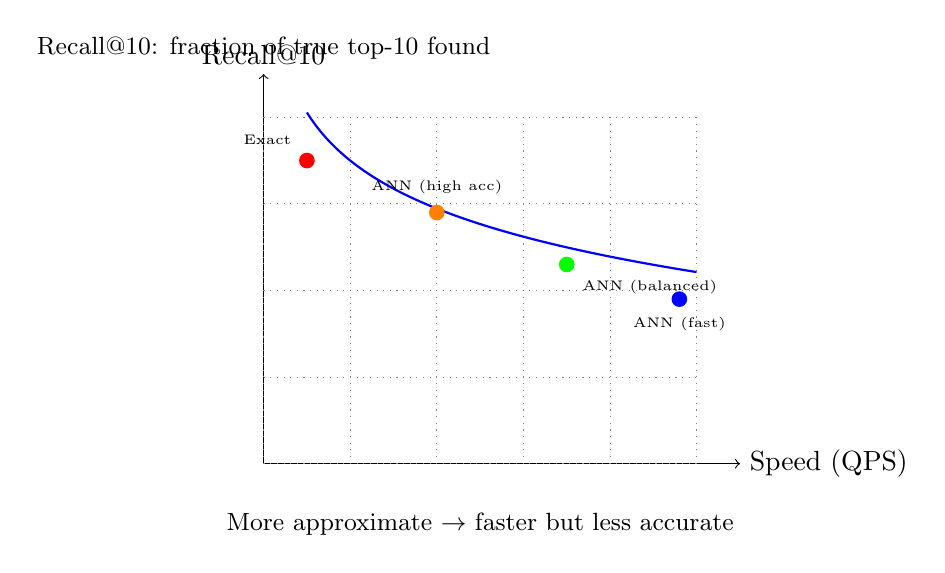
\begin{tikzpicture}[scale=1.1]
    % Axes
    \draw[->] (0,0) -- (5.5,0) node[right] {Speed (QPS)};
    \draw[->] (0,0) -- (0,4.5) node[above] {Recall@10};
    
    % Grid
    \draw[gray, dotted] (0,0) grid (5,4);
    
    % Line showing trade-off
    \draw[blue, thick, domain=0.5:5, samples=100] 
        plot (\x, {3.5 - 0.8*ln(\x)});
    
    % Points on curve
    \node[circle, fill=red, inner sep=2pt, label=above left:{\tiny Exact}] at (0.5, 3.5) {};
    \node[circle, fill=orange, inner sep=2pt, label=above:{\tiny ANN (high acc)}] at (2, 2.9) {};
    \node[circle, fill=green, inner sep=2pt, label=below right:{\tiny ANN (balanced)}] at (3.5, 2.3) {};
    \node[circle, fill=blue, inner sep=2pt, label=below:{\tiny ANN (fast)}] at (4.8, 1.9) {};
    
    % Labels
    \node at (2.5, -0.7) {\small More approximate $\rightarrow$ faster but less accurate};
    \node at (0, 4.8) {\small Recall@10: fraction of true top-10 found};
\end{tikzpicture}
\end{center}

\vspace{1em}

\textbf{Typical operating points:}
\begin{itemize}
    \item High accuracy: 95-99\% recall, 100-500 QPS
    \item Balanced: 90-95\% recall, 500-2000 QPS
    \item Fast: 80-90\% recall, 2000-10000 QPS
\end{itemize}
\end{frame}

\begin{frame}{Main ANN Approaches}
\begin{enumerate}
    \item \textbf{Graph-Based} (HNSW, NSG)
    \begin{itemize}
        \item Build graph connecting similar vectors
        \item Search by navigating graph
        \item High accuracy, moderate memory
    \end{itemize}
    
    \item \textbf{Clustering/Inverted File (IVF, IMI)}
    \begin{itemize}
        \item Cluster vectors (k-means)
        \item Search only in nearest clusters
        \item Fast, lower accuracy
    \end{itemize}
    
    \item \textbf{Product Quantization (PQ)}
    \begin{itemize}
        \item Compress vectors aggressively
        \item Approximate distances in compressed space
        \item Very memory-efficient
    \end{itemize}
    
    \item \textbf{Tree-Based} (Annoy, KD-tree)
    \begin{itemize}
        \item Partition space with trees
        \item Search by tree traversal
        \item Simple, good for moderate dimensions
    \end{itemize}
    
    \item \textbf{Hashing} (LSH)
    \begin{itemize}
        \item Hash similar vectors to same buckets
        \item Search in hash buckets
        \item Fast but less accurate
    \end{itemize}
\end{enumerate}
\end{frame}

\begin{frame}{HNSW: Hierarchical Navigable Small World}
\begin{block}{Core Idea}
Build a multi-layer graph where upper layers provide "highways" for fast navigation to the target region
\end{block}

\vspace{1em}

\begin{center}
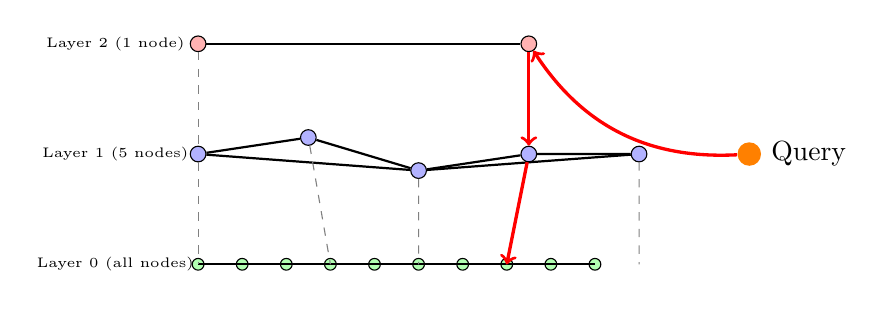
\begin{tikzpicture}[scale=0.7]
    % Layer 2 (top, sparse)
    \node[circle, draw, fill=red!30, inner sep=2pt] (t1) at (0,5) {};
    \node[circle, draw, fill=red!30, inner sep=2pt] (t2) at (6,5) {};
    \draw[thick] (t1) -- (t2);
    \node at (-1.5,5) {\tiny Layer 2 (1 node)};
    
    % Layer 1 (middle)
    \node[circle, draw, fill=blue!30, inner sep=2pt] (m1) at (0,3) {};
    \node[circle, draw, fill=blue!30, inner sep=2pt] (m2) at (2,3.3) {};
    \node[circle, draw, fill=blue!30, inner sep=2pt] (m3) at (4,2.7) {};
    \node[circle, draw, fill=blue!30, inner sep=2pt] (m4) at (6,3) {};
    \node[circle, draw, fill=blue!30, inner sep=2pt] (m5) at (8,3) {};
    
    \draw[thick] (m1) -- (m2) -- (m3) -- (m4) -- (m5);
    \draw[thick] (m1) -- (m3);
    \draw[thick] (m3) -- (m5);
    
    \draw[dashed, gray] (t1) -- (m1);
    \draw[dashed, gray] (t2) -- (m4);
    \node at (-1.5,3) {\tiny Layer 1 (5 nodes)};
    
    % Layer 0 (bottom, dense)
    \foreach \x in {0,0.8,...,8} {
        \node[circle, draw, fill=green!30, inner sep=1.5pt] at (\x,1) {};
    }
    
    % Connections at layer 0 (simplified)
    \foreach \x in {0,0.8,...,7.2} {
        \pgfmathsetmacro{\nextx}{\x+0.8}
        \draw[thick] (\x,1) -- (\nextx,1);
    }
    
    \draw[dashed, gray] (m1) -- (0,1);
    \draw[dashed, gray] (m2) -- (2.4,1);
    \draw[dashed, gray] (m3) -- (4,1);
    \draw[dashed, gray] (m4) -- (5.6,1);
    \draw[dashed, gray] (m5) -- (8,1);
    
    \node at (-1.5,1) {\tiny Layer 0 (all nodes)};
    
    % Query path
    \node[circle, fill=orange, inner sep=3pt, label=right:Query] (q) at (10,3) {};
    \draw[->, red, very thick] (q) to[bend left] (t2);
    \draw[->, red, very thick] (t2) -- (m4);
    \draw[->, red, very thick] (m4) -- (5.6,1);
\end{tikzpicture}
\end{center}

\textbf{Search:} Start at top, greedily navigate to nearest neighbor at each layer, descend to next layer, repeat
\end{frame}

\begin{frame}{HNSW: Construction}
\begin{algorithmic}[1]
\STATE \textbf{Input:} Set of vectors $V$, parameter $M$ (max connections per node)
\STATE \textbf{Output:} Multi-layer graph
\STATE
\STATE Initialize empty graph
\FOR{each vector $\vec{v}$ in $V$}
    \STATE $\ell \gets$ random layer (exponentially decaying probability)
    \STATE Insert $\vec{v}$ at layer $\ell$ and all layers below
    \FOR{each layer from top to $\ell$}
        \STATE Find $M$ nearest neighbors at this layer (using greedy search)
        \STATE Connect $\vec{v}$ to these neighbors
        \IF{neighbor has > $M$ connections}
            \STATE Prune least useful edge
        \ENDIF
    \ENDFOR
\ENDFOR
\RETURN Multi-layer graph
\end{algorithmic}

\vspace{1em}

\textbf{Key parameters:}
\begin{itemize}
    \item $M$: Max connections (typical: 16-64)
    \item $efConstruction$: Search width during construction (typical: 100-200)
\end{itemize}
\end{frame}

\begin{frame}{HNSW: Search}
\begin{algorithmic}[1]
\STATE \textbf{Input:} Query $\vec{q}$, graph $G$, $k$ (neighbors to find), $ef$ (search width)
\STATE \textbf{Output:} Approximate $k$ nearest neighbors
\STATE
\STATE $\text{currLayer} \gets$ top layer
\STATE $\text{entryPoint} \gets$ entry node at top layer
\STATE $\text{candidates} \gets$ priority queue (min-heap by distance)
\STATE $\text{visited} \gets$ set of visited nodes
\WHILE{$\text{currLayer} \geq 0$}
    \STATE Add $\text{entryPoint}$ to candidates and visited
    \WHILE{candidates not empty}
        \STATE $\text{nearest} \gets$ pop closest unvisited from candidates
        \FOR{each neighbor $n$ of $\text{nearest}$ at $\text{currLayer}$}
            \IF{$n$ not in visited}
                \STATE Add $n$ to candidates and visited
                \IF{distance($\vec{q}$, $n$) < distance to farthest in top-$ef$}
                    \STATE Keep $n$ in top-$ef$ candidates
                \ENDIF
            \ENDIF
        \ENDFOR
    \ENDWHILE
    \STATE $\text{entryPoint} \gets$ closest candidate
    \STATE $\text{currLayer} \gets \text{currLayer} - 1$
\ENDWHILE
\RETURN top-$k$ from candidates
\end{algorithmic}
\end{frame}

\begin{frame}{HNSW: Properties}
\begin{block}{Advantages}
\begin{itemize}
    \item \textcolor{green}{\checkmark} Excellent recall (95-99\% typical)
    \item \textcolor{green}{\checkmark} Fast search: $O(\log N)$ average
    \item \textcolor{green}{\checkmark} Supports updates (add/delete vectors)
    \item \textcolor{green}{\checkmark} No training required
    \item \textcolor{green}{\checkmark} Works well in high dimensions (100-1000d)
\end{itemize}
\end{block}

\begin{alertblock}{Disadvantages}
\begin{itemize}
    \item \textcolor{red}{\ding{55}} High memory usage (graph structure: $\approx 2\times$ vector size)
    \item \textcolor{red}{\ding{55}} Slower to build than some alternatives
    \item \textcolor{red}{\ding{55}} Not as memory-efficient as quantization methods
\end{itemize}
\end{alertblock}

\vspace{1em}

\textbf{When to use:}
\begin{itemize}
    \item High recall critical (e.g., production search)
    \item Sufficient memory available
    \item Dynamic index (frequent updates)
\end{itemize}
\end{frame}

\begin{frame}{IVF: Inverted File Index}
\begin{block}{Core Idea}
Cluster vectors with k-means, then search only in nearest clusters
\end{block}

\vspace{1em}

\begin{center}
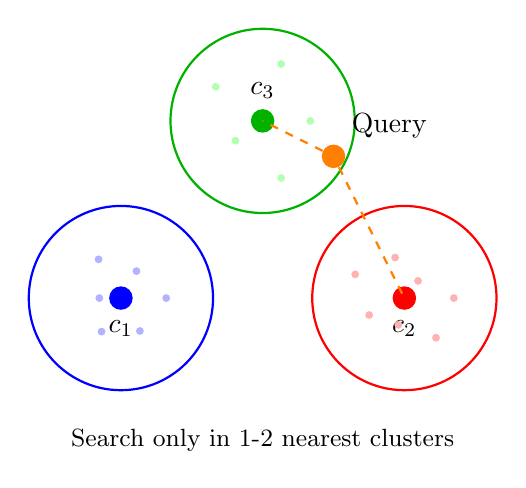
\begin{tikzpicture}[scale=0.9]
    % Cluster 1
    \draw[thick, blue] (0,0) circle (1.3);
    \node[circle, fill=blue, inner sep=3pt, label=below:$c_1$] at (0,0) {};
    \foreach \i in {1,...,6} {
        \pgfmathsetmacro{\angle}{60*\i}
        \pgfmathsetmacro{\r}{0.3+0.4*rnd}
        \node[circle, fill=blue!30, inner sep=1pt] at (\angle:\r) {};
    }
    
    % Cluster 2
    \draw[thick, red] (4,0) circle (1.3);
    \node[circle, fill=red, inner sep=3pt, label=below:$c_2$] at (4,0) {};
    \foreach \i in {1,...,7} {
        \pgfmathsetmacro{\angle}{360/7*\i}
        \pgfmathsetmacro{\r}{0.3+0.5*rnd}
        \node[circle, fill=red!30, inner sep=1pt] at ($(4,0)+(\angle:\r)$) {};
    }
    
    % Cluster 3
    \draw[thick, green!70!black] (2,2.5) circle (1.3);
    \node[circle, fill=green!70!black, inner sep=3pt, label=above:$c_3$] at (2,2.5) {};
    \foreach \i in {1,...,5} {
        \pgfmathsetmacro{\angle}{72*\i}
        \pgfmathsetmacro{\r}{0.4+0.5*rnd}
        \node[circle, fill=green!30, inner sep=1pt] at ($(2,2.5)+(\angle:\r)$) {};
    }
    
    % Query
    \node[circle, fill=orange, inner sep=3pt, label=above right:Query] (q) at (3,2) {};
    
    % Distance to nearest cluster
    \draw[dashed, orange, thick] (q) -- (2,2.5);
    \draw[dashed, orange, thick] (q) -- (4,0);
    
    \node at (2,-2) {\small Search only in 1-2 nearest clusters};
\end{tikzpicture}
\end{center}

\textbf{Steps:}
\begin{enumerate}
    \item Offline: Cluster all vectors (e.g., $k=1000$ clusters)
    \item Online: Find $n_{probe}$ nearest cluster centers to query
    \item Search exhaustively within those clusters
    \item Merge and return top-$k$
\end{enumerate}
\end{frame}

\begin{frame}[shrink=10]{IVF: Algorithm Details}
\textbf{Index Construction:}
\begin{algorithmic}[1]
\STATE Run k-means on all vectors $\rightarrow$ get $k$ cluster centers $\{c_1, \ldots, c_k\}$
\STATE Assign each vector to its nearest cluster center
\STATE Build inverted lists: cluster $i$ $\rightarrow$ list of vectors in that cluster
\end{algorithmic}

\vspace{1em}

\textbf{Search:}
\begin{algorithmic}[1]
\STATE \textbf{Input:} Query $\vec{q}$, $n_{probe}$ (clusters to search), $k$ (neighbors)
\STATE Compute distance from $\vec{q}$ to all cluster centers
\STATE Select $n_{probe}$ nearest cluster centers
\STATE $\text{candidates} \gets []$
\FOR{each selected cluster}
    \STATE Fetch all vectors in cluster
    \STATE Compute exact distances to $\vec{q}$
    \STATE Add to candidates
\ENDFOR
\STATE Sort candidates by distance
\RETURN top-$k$ candidates
\end{algorithmic}

\vspace{1em}

\textbf{Key parameter:} $n_{probe}$ (trade recall for speed)
\begin{itemize}
    \item $n_{probe} = 1$: Fast but low recall (search 1 cluster)
    \item $n_{probe} = 10$: Balanced (search 10 clusters)
    \item $n_{probe} = k$: Exact search (search all clusters)
\end{itemize}
\end{frame}

\begin{frame}[shrink=10]{Product Quantization (PQ)}
\begin{block}{Goal}
Compress vectors aggressively while preserving distance relationships
\end{block}

\vspace{1em}

\textbf{Key idea:}
\begin{enumerate}
    \item Split each $d$-dimensional vector into $m$ subvectors ($d/m$ dims each)
    \item Quantize each subvector independently using k-means
    \item Represent vector as $m$ cluster IDs (e.g., $m$ bytes)
\end{enumerate}

\vspace{1em}

\begin{exampleblock}{Example}
\textbf{Original:} 768-dim vector (768 $\times$ 4 bytes = 3072 bytes) \\
\textbf{PQ compression:}
\begin{itemize}
    \item Split into $m=96$ subvectors of 8 dims each
    \item Quantize each subvector to $k=256$ centroids (1 byte ID)
    \item Compressed: 96 bytes (32$\times$ compression!)
\end{itemize}
\end{exampleblock}

\vspace{1em}

\textbf{Distance computation:}
\begin{itemize}
    \item Pre-compute distances from query subvectors to all centroids
    \item Approximate distance = sum of subvector distances (lookup table)
    \item Very fast! (just $m$ additions)
\end{itemize}
\end{frame}

\begin{frame}{PQ: Detailed Algorithm}
\textbf{Training:}
\begin{algorithmic}[1]
\STATE Split each vector into $m$ subvectors of dimension $d/m$
\FOR{each subspace $i = 1, \ldots, m$}
    \STATE Run k-means on all subvectors in subspace $i$ $\rightarrow$ get $k$ centroids
    \STATE Store these centroids as codebook $\mathcal{C}_i$
\ENDFOR
\end{algorithmic}

\vspace{1em}

\textbf{Encoding:}
\begin{algorithmic}[1]
\STATE \textbf{Input:} Vector $\vec{v}$
\STATE Split $\vec{v}$ into subvectors $[\vec{v}_1, \vec{v}_2, \ldots, \vec{v}_m]$
\FOR{each subvector $\vec{v}_i$}
    \STATE Find nearest centroid in $\mathcal{C}_i$ $\rightarrow$ get ID $c_i$
\ENDFOR
\STATE Store vector as $[c_1, c_2, \ldots, c_m]$ (m bytes if k=256)
\end{algorithmic}

\vspace{1em}

\textbf{Search:}
\begin{algorithmic}[1]
\STATE Split query $\vec{q}$ into subvectors $[\vec{q}_1, \ldots, \vec{q}_m]$
\STATE For each subspace $i$, compute distance table: $\vec{q}_i$ to all centroids in $\mathcal{C}_i$
\FOR{each encoded vector $[c_1, \ldots, c_m]$}
    \STATE Approximate distance = $\sum_{i=1}^{m} \text{distTable}_i[c_i]$ (m lookups)
\ENDFOR
\STATE Return top-$k$ by approximate distance
\end{algorithmic}
\end{frame}

\begin{frame}[shrink=10]{IVF + PQ: Best of Both Worlds}
\begin{block}{IVFPQ: Combine IVF with Product Quantization}
\begin{enumerate}
    \item Use IVF for coarse filtering (cluster-level search)
    \item Use PQ for compression within clusters
    \item Get both speed (IVF) and memory efficiency (PQ)
\end{enumerate}
\end{block}

\vspace{1em}

\textbf{Algorithm:}
\begin{enumerate}
    \item Offline: Cluster vectors into $k$ clusters (IVF)
    \item Offline: Within each cluster, train PQ codebooks
    \item Offline: Encode all vectors with PQ
    \item Online: Find $n_{probe}$ nearest clusters
    \item Online: Search within those clusters using PQ distances
\end{enumerate}

\vspace{1em}

\textbf{Memory savings example:}
\begin{itemize}
    \item Original: 1B vectors $\times$ 768 dims $\times$ 4 bytes = 3TB
    \item IVFPQ: 1B vectors $\times$ 64 bytes (PQ) = 64GB
    \item \textbf{50$\times$ compression!}
\end{itemize}

\vspace{1em}

\textbf{Trade-off:} Lower recall than HNSW, but much more memory-efficient
\end{frame}

\begin{frame}[shrink=5]{ANN Libraries Comparison}
\begin{table}
\centering
\tiny
\begin{tabular}{lccccc}
\toprule
\textbf{Library} & \textbf{Method} & \textbf{Recall} & \textbf{Speed} & \textbf{Memory} & \textbf{Updates} \\
\midrule
HNSW (hnswlib) & Graph & Excellent & Fast & High & Yes \\
FAISS (IVF) & Clustering & Good & Very Fast & Medium & Limited \\
FAISS (IVFPQ) & Clustering+PQ & Good & Very Fast & Low & Limited \\
FAISS (HNSW) & Graph & Excellent & Fast & High & Yes \\
Annoy & Trees & Good & Fast & Medium & No \\
ScaNN & Learned quant. & Excellent & Very Fast & Low & Limited \\
Milvus & Multiple & Excellent & Fast & Varies & Yes \\
Weaviate & HNSW & Excellent & Fast & High & Yes \\
\bottomrule
\end{tabular}
\end{table}

\vspace{1em}

\begin{block}{Choosing a Library}
\begin{itemize}
    \item \textbf{High recall needed:} HNSW (hnswlib, Weaviate)
    \item \textbf{Memory constrained:} FAISS IVFPQ, ScaNN
    \item \textbf{Maximum speed:} FAISS IVF (lower recall)
    \item \textbf{Distributed/production:} Milvus, Weaviate, Qdrant
    \item \textbf{Simple/prototyping:} Annoy, hnswlib
\end{itemize}
\end{block}
\end{frame}

\begin{frame}{Hybrid: Sparse + Dense}
\begin{block}{Why Hybrid?}
Sparse and dense retrieval have complementary strengths
\end{block}

\vspace{1em}

\begin{columns}
\begin{column}{0.48\textwidth}
\textbf{Sparse (BM25) strengths:}
\begin{itemize}
    \item Exact term matching
    \item Rare/specific terms
    \item Named entities
    \item Acronyms, IDs
    \item Explainable
\end{itemize}
\end{column}

\begin{column}{0.48\textwidth}
\textbf{Dense strengths:}
\begin{itemize}
    \item Semantic matching
    \item Synonyms
    \item Paraphrases
    \item Conceptual similarity
    \item Cross-lingual
\end{itemize}
\end{column}
\end{columns}

\vspace{1em}

\textbf{Hybrid approaches:}
\begin{enumerate}
    \item \textbf{Parallel retrieval + fusion}
    \begin{itemize}
        \item Run sparse and dense in parallel
        \item Merge results (e.g., reciprocal rank fusion)
    \end{itemize}
    
    \item \textbf{Cascade: Sparse $\rightarrow$ Dense}
    \begin{itemize}
        \item Stage 1: BM25 retrieves 1000 candidates
        \item Stage 2: Dense re-ranks top 1000
    \end{itemize}
    
    \item \textbf{Learned combination}
    \begin{itemize}
        \item Use both sparse and dense scores as features
        \item Learn optimal combination (Lecture 6: LTR)
    \end{itemize}
\end{enumerate}
\end{frame}

% ====================================================================
% WRAP-UP
% ====================================================================
\section{Summary}

\begin{frame}{Key Takeaways: Posting Lists}
\begin{enumerate}
    \item \textbf{Posting list structure}
    \begin{itemize}
        \item Core: (docID, frequency, positions)
        \item Sorted by docID for merge operations
        \item Variable length (power-law distribution)
    \end{itemize}
    
    \item \textbf{Skip lists}
    \begin{itemize}
        \item Add "highways" for faster intersection
        \item Place every $\sqrt{n}$ elements typically
        \item Trade space for speed
    \end{itemize}
\end{enumerate}
\end{frame}

\begin{frame}{Key Takeaways: Query Processing}
\begin{enumerate}
    \item \textbf{DAAT vs. TAAT}
    \begin{itemize}
        \item DAAT: Process one document at a time (modern systems)
        \item TAAT: Process one term at a time (batch scoring)
    \end{itemize}
    
    \item \textbf{Optimizations}
    \begin{itemize}
        \item MaxScore: Skip low-impact terms
        \item WAND: Dynamic pruning with upper bounds
        \item Impact-ordered indexes: Early termination
    \end{itemize}
\end{enumerate}
\end{frame}

\begin{frame}{Key Takeaways: Compression}
\begin{enumerate}
    \item \textbf{Gap encoding is essential}
    \begin{itemize}
        \item Store gaps instead of absolute docIDs
        \item Most gaps are small (compress well)
    \end{itemize}
    
    \item \textbf{Compression methods}
    \begin{itemize}
        \item VB: Simple, fast, 3-4$\times$ compression
        \item Gamma: Better for small numbers
        \item PForDelta: Best performance, 6-10$\times$ compression
    \end{itemize}
    
    \item \textbf{Why it matters}
    \begin{itemize}
        \item Smaller index $\rightarrow$ fits in RAM
        \item Faster I/O $\rightarrow$ better query latency
        \item Disk is slow, CPU is fast
    \end{itemize}
\end{enumerate}
\end{frame}

\begin{frame}{Key Takeaways: ANN Indexing}
\begin{enumerate}
    \item \textbf{Dense retrieval requires ANN}
    \begin{itemize}
        \item Exact search too slow for billion-scale
        \item Trade recall for speed (90-99\% recall acceptable)
    \end{itemize}
    
    \item \textbf{Main approaches}
    \begin{itemize}
        \item HNSW: Graph-based, excellent recall
        \item IVF: Clustering, fast but needs more probes
        \item PQ: Aggressive compression, memory-efficient
        \item IVFPQ: Combines IVF + PQ (production standard)
    \end{itemize}
    
    \item \textbf{Hybrid is often best}
    \begin{itemize}
        \item Sparse for exact matching
        \item Dense for semantic matching
        \item Combine for best of both worlds
    \end{itemize}
\end{enumerate}
\end{frame}

\begin{frame}{The Complete Modern IR Stack}
\begin{center}
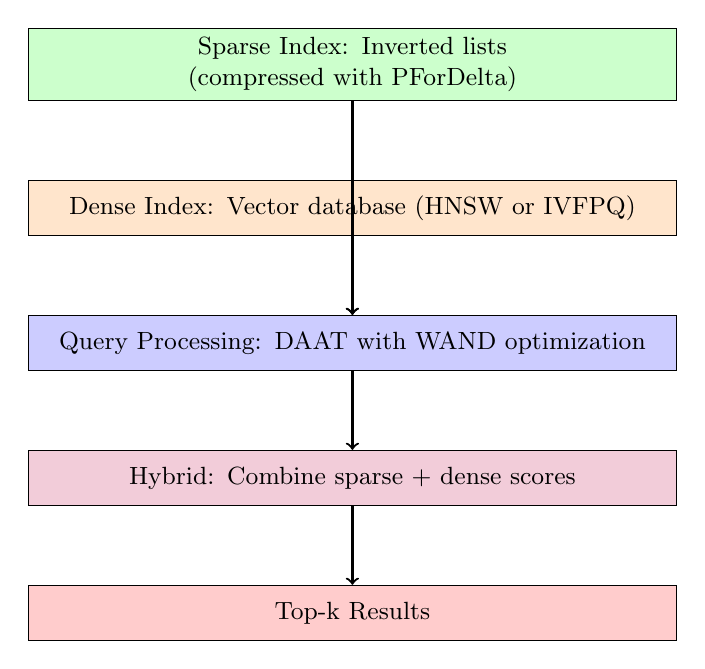
\begin{tikzpicture}[
    node distance=1cm,
    box/.style={rectangle, draw, fill=blue!20, text width=8cm, align=center, minimum height=0.7cm, font=\small},
    arrow/.style={->, thick}
]
    \node[box, fill=green!20] (sparse) {Sparse Index: Inverted lists (compressed with PForDelta)};
    \node[box, below=of sparse, fill=orange!20] (dense) {Dense Index: Vector database (HNSW or IVFPQ)};
    \node[box, below=of dense] (query) {Query Processing: DAAT with WAND optimization};
    \node[box, below=of query, fill=purple!20] (hybrid) {Hybrid: Combine sparse + dense scores};
    \node[box, below=of hybrid, fill=red!20] (results) {Top-k Results};
    
    \draw[arrow] (sparse) -- (query);
    \draw[arrow] (dense) -- (query);
    \draw[arrow] (query) -- (hybrid);
    \draw[arrow] (hybrid) -- (results);
\end{tikzpicture}
\end{center}

\vspace{1em}

\textbf{This is what powers modern search engines!}
\end{frame}

\begin{frame}{Questions?}
\begin{center}
\Huge Thank you!

\vspace{2em}

\Large Questions?

\vspace{2em}

\normalsize
\textbf{Next: Lecture 3 — Ranking Models}

We'll use these indexes to implement BM25, language models, \\
and query expansion with RM3!
\end{center}
\end{frame}

\end{document}
